\documentclass{mwart}
\usepackage[utf8]{inputenc}
\usepackage{polski}
\usepackage{amsmath,amssymb}
\usepackage[margin=2cm]{geometry}
\usepackage{tikz}
\pagestyle{empty}
\linespread{1.3}
\newcommand{\ans}[1]{}
\begin{document}
\section{Przestrzeń probabilistyczna}
\begin{enumerate}
\item Na ile sposobów można ustawić 5 osób w kolejce? \ans{$5!$}
\item Ile słów pięcioliterowych (nawet tych bezsensownych) można utworzyć z liter \emph{A, B, C}? \ans{$3^5=243$}
\item Dane są dwa pojemniki. W pierwszym z nich znajduje się 11 kul: 7 białych i 4 czarne. W~drugim pojemniku jest 6 kul: 3 białe i 3 czarne. Z każdego pojemnika losujemy po dwie kule.
Rozpatrz poniższe pytania w dwóch wariantach: wszystkie kule w danym kolorze są identyczne oraz gdy kule są rozróżnialne (np. numerowane).
\begin{enumerate}
\item Ile jest możliwych układów? \ans{${11 \choose 2}{6 \choose 2}=825$}
\item Ile jest układów składających się wyłącznie z kul czarnych? \ans{${4 \choose 2}{3 \choose 2}=18$}
\item Ile jest układów składających się wyłącznie z kul białych? \ans{${7 \choose 2}{3 \choose 2}=63$}
\item Ile jest układów składających się z pary białej i pary czarnej? \ans{${7\choose 2}{3 \choose 2}+{4 \choose 2}{3 \choose 2}+7\cdot4\cdot3\cdot3=333$}
\item Ile jest układów składających się z jednej kuli białej i trzech czarnych? \ans{$7\cdot4\cdot{3\choose 2}+3\cdot3\cdot{4\choose 2}=138$}
\item Ile jest układów składających się z jednej kuli czarnej i trzech białych?  \ans{$4\cdot7\cdot{3\choose 2}+3\cdot3\cdot{7\choose 2}=273$}
\end{enumerate}
\item Z partii towaru zawierającej sztuki dobre i niedobre losujemy 3 sztuki (\emph{próba}). Niech $A$ oznacza zdarzenie: \emph{dokładnie jedna sztuka dobra w próbie}, $B$ zdarzenie: \emph{co najwyżej jedna sztuka dobra w próbie}, $C$ zdarzenie: \emph{co najmniej jedna sztuka dobra w próbie}. Opisz słownie następujące zdarzenia:
\begin{enumerate}
\item $A'$, $B'$, $C'$
\item $A\cup B$
\item $A\cap B$
\item $B\cup C$
\item $B\cap C$
\item $B'\cap C'$
\end{enumerate}
\item Inżynier projektuje magazyn do przechowywania kartonów puszek żywności. Kartony mają kształt sześcianów o krawędzi 4 dm i masie 50 kg każdy. Zakłada się, że kartony nie mogą być ułożone w wieżę wyższą niż 24 dm. Zaproponować przestrzeń zdarzeń losowych dla następujących doświadczeń:
\begin{enumerate}
\item Obserwacja całkowitego obciążenia 16 $dm^2$ powierzchni pochodzącego z jednego stosu kartonów.
\item Obserwacja całkowitego obciążenia 16 $dm^2$ powierzchni pochodzącego z dwóch stosów kartonów, przy założeniu, że jest to obciążenie wywołane przezpolowę masy każdego z dwóch stosów.
\end{enumerate}
W obu przestrzeniach opisać następujące zdarzenia:
\begin{description}
\item[A] całkowite obciążenie wynosi co najmniej 150 kg;
\item[B] całkowite obciążenie wynosi nie więcej niż 200 kg;
\item[C] całkowite obciążenie przekracza 250 kg;
\end{description}
\item  Drewniane pale mają losową długość $L$ nie przekraczającą 12 m. Pale są przeznaczone do wbijania w ziemię, której skalna warstwa stanowiąca opór znajduje się na losowej głębokości $H$, nie większej niż 10 m. Zaproponować przestrzeń zdarzeń elementarnych dla tak opisanego doświadczenia. Zdefiniować przez odpowiednie zdarzenia elementarne następujące doświadczenia:
\begin{description}
\item[A] długość losowo wybranego pala będzie większa od głębokości skalnej warstwy;
\item[B] głębkość skalnej warstwy przekroczy 8 metrów;
\item[C] długość losowo wybranego pala przekroczy 8 metrów;
\item[D] $B\cap C$
\item[E] $B\cup C$
\item[F] $(B\cup C)\cap A'$
\end{description}
\item Na 10 kartkach napisano liczby od 1 do 10 i wrzucono do pudełka. Losujemy w sposób przypadkowy dwie kartki. Niech $A$ odpowiada zdarzeniu \emph{wylosowanie kartki z numerem 1}, a $B$ zdarzeniu \emph{wylosowanie pary liczb, których suma jest większa od 4}. Zakładamy, że wylosowanie każdej z kartek jest równoprawdopodobne.
\begin{enumerate}
\item Przedstaw przestrzeń zdarzeń elementarnych. Podaj jej rozmiar. \ans{$\Omega=\{\omega_{\{i,j\}}|i,j\in\{1,\ldots,10\} \land i\neq j\}, \left|\Omega\right|={10 \choose 2}=45$}
\item Zdefiniuj zdarzenia $A$ i $B$ jako zbiory zdarzeń elementarnych. \ans{$A=\{\omega_{\{i,j\}}\in\Omega|i=1 \lor j=1\}$, $B=\{\omega_{\{i,j\}}\in\Omega|i+j>4\}$}
\item Ile jest zdarzeń sprzyjających zdarzeniom $A$ i $B$. \ans{$\left|A\right|=9$, $\left|B\right|=45-4=41$}
\item Oblicz $P(A)$ i $P(B)$ \ans{$P(A)=\frac{9}{45}, P(B)=\frac{41}{45}$}
\end{enumerate}
\item W gospodzie \emph{Złoty okoń} zorganizowano loterię, w której do sprzedania było 100 biletów, a wygrywał tylko jeden. Każdy mógł kupić najwyżej jeden bilet. Niech zdarzenie $A$ odpowiada sytuacji, w której Estella posiada los wygrywający. Jakie ma szanse na wygraną?
\begin{enumerate}%
\item Przedstaw przestrzeń zdarzeń elementarnych. \ans{$\Omega=\{\omega_n|n=1,2,\ldots,100\}$}%
\item Czy w tej przestrzeni wszystkie zdarzenia elementarne są jednakowo prawdopodobne? \ans{Tak}%
\item Jaki jest rozmiar przestrzeni zdarzeń elementarnych? \ans{$\left|\Omega\right|=100$}%
\item Zdefiniuj zdarzenie $A$ jako zbiór zdarzeń elementarnych. \ans{$A=\{\omega_1$\}}%
\item Oblicz prawdpodobieństwo $P(A)$, dbając o to by jasno przedstawić tok rozumowania. \ans{$P(A)=\frac{1}{100}$}%
\end{enumerate}%
\item W gospodzie \emph{Pod Zielonym Smokiem} oferują sześć różnych dań obiadowych. Pięciu klientów wchodzi jeden po drugim do gospody
i~niezależnie od siebie zamawia posiłek. Niech zdarzenie $A$ odpowiada sytuacji, w~której pierwsze danie z menu zamówi dokładnie jedna osoba.%
\begin{enumerate}%
\item Przedstaw przestrzeń zdarzeń elementarnych. \ans{$\Omega=\{\omega_{i_1,\ldots,i_5}|i_j=1,2,\ldots,6\}$}%
\item Czy w tej przestrzeni wszystkie zdarzenia elementarne są jednakowo prawdopodobne? \ans{Tak}%
\item Jaki jest rozmiar przestrzeni zdarzeń elementarnych? \ans{$\left|\Omega\right|=6^5$}%
\item Zdefiniuj zdarzenie $A$ jako zbiór zdarzeń elementarnych. \ans{$A=\{\omega_{i_1,\ldots,i_5}|\exists j: i_j=1 \land \forall k\neq j: i_k\neq 1\}$, $\left|A\right|=5\cdot5^4$}%
\item Oblicz prawdpodobieństwo $P(A)$, dbając o to by jasno przedstawić tok rozumowania. \ans{$P(A)=\frac{5^5}{6^5}=\frac{5}{6}^5\approx 0{,}40$}%
\end{enumerate}%
\end{enumerate}
\clearpage
\section{Przestrzeń probabilistyczna -- zadania dodatkowe}
\begin{enumerate}
\item Oblicz, ile jest liczb naturalnych sześciocyfrowych, w zapisie których występuje dokładnie trzy razy cyfra 0 i dokładnie raz występuje cyfra 5. \ans{${8\choose 2}3\frac{5!}{3!}+8\cdot\left(\frac{5!}{3!2!}+\frac{5!}{3!}\right)=1920$}
\item Partia towaru składa się ze 100 elementów, wśród których 5 jest wadliwych. Poddajemy kontroli 50 elementów. Partię przyjmujemy, jeśli wśród kontrolowanych elementów jest nie więcej niż jeden wadliwy. Niech zdarzenie $A$ odpowiada przyjęciu partii.
\begin{enumerate}%
\item Przedstaw przestrzeń zdarzeń elementarnych. \ans{$\Omega=\{\omega_J|\left|J\right|=50 \land J\subset\{1,2,\ldots,100\}\}$}%
\item Czy w tej przestrzeni wszystkie zdarzenia elementarne są jednakowo prawdopodobne? \ans{Tak}%
\item Jaki jest rozmiar przestrzeni zdarzeń elementarnych? \ans{$\left|\Omega\right|={100\choose 50}$}%
\item Zdefiniuj zdarzenie $A$ jako zbiór zdarzeń elementarnych. \ans{$A=\{\omega_J|\left|J\cap \{1,2,\ldots,5\}\right|\leq 1\}$}%
\item Oblicz prawdpodobieństwo $P(A)$, dbając o to by jasno przedstawić tok rozumowania. \ans{$\left|A\right|={5\choose 1}{95\choose 49}+{95\choose 50}, P(A)\approx0{,}181$}%
\end{enumerate}%
\item Winda rusza z siedmioma pasażerami i zatrzymuje się na dziesięciu piętrach. Niech zdarzenie $A$ odpowiada sytuacji, w której żadnych dwóch pasażerów nie opuści windy na tym samym piętrze.
\begin{enumerate}%
\item Przedstaw przestrzeń zdarzeń elementarnych. \ans{$\Omega=\{\omega_{i_1,\ldots,i_7}|i_j=1,2,\ldots,10\}$}%
\item Czy w tej przestrzeni wszystkie zdarzenia elementarne są jednakowo prawdopodobne? \ans{Tak}%
\item Jaki jest rozmiar przestrzeni zdarzeń elementarnych? \ans{$\left|\Omega\right|=10^7$}%
\item Zdefiniuj zdarzenie $A$ jako zbiór zdarzeń elementarnych. \ans{$A=\{\omega_{i_1,\ldots,i_7}|\forall j,k\colon j\neq k\to i_j\neq i_k\}, \left|A\right|=\frac{10!}{3!}=604800$}%
\item Oblicz prawdpodobieństwo $P(A)$, dbając o to by jasno przedstawić tok rozumowania. \ans{$P(A)=\frac{604800}{10^7}=0{,}06$}%
\end{enumerate}%
\item Dwudziestoosobowa grupa studencka, w której jest 6 kobiet, otrzymała 5 biletów do teatru. Bilety rozdziela się drogą losowania. Niech zdarzenie $A$ odpowiada sytuacji, w której wśród posiadaczy biletów znajdą się dokładnie trzy kobiety.
\begin{enumerate}%
\item Przedstaw przestrzeń zdarzeń elementarnych. \ans{$\Omega=\{\omega_J|\left|J\right|=5 \land J\subset\{1,2,\ldots,20\}\}$}%
\item Czy w tej przestrzeni wszystkie zdarzenia elementarne są jednakowo prawdopodobne? \ans{Tak}%
\item Jaki jest rozmiar przestrzeni zdarzeń elementarnych? \ans{$\left|\Omega\right|={20\choose 5}=15504$}%
\item Zdefiniuj zdarzenie $A$ jako zbiór zdarzeń elementarnych. \ans{$A=\{\omega_J|\left|J\cap \{1,2,\ldots,6\}\right|=3\}, \left|A\right|={6\choose 3}{14\choose 2}=1820$}%
\item Oblicz prawdpodobieństwo $P(A)$, dbając o to by jasno przedstawić tok rozumowania. \ans{$P(A)=0{,}12$}%
\end{enumerate}%
\end{enumerate}%
\clearpage
\section{Prawdopodobieństwo warunkowe i niezależność zdarzeń}
\begin{enumerate}
\item W sklepie są sprzedawane baterie dwóch firm A i B. Firma A dostarcza do sklepu dwa razy więcej baterii niż firma B. Braki wśród baterii tych firm stanowią odpowiednio $0{,}9\%$ i $1{,}4\%$. Kupujemy jedną baterię. Jakie jest prawdopodobieństwo kupienia baterii dobrej?
\item Wiadomo, że 90\% produkcji spełnia wymagania techniczne. Przeprowadzono dodatkową kontrolę, przy której mogły być popełnione pewne błędy, a mianowicie: element wadliwy mógł zostać sklasyfikowany jako dobry z prawdopodobieństwem $0{,}05$, a element dobry mógł zostać sklasyfikowany jako wadliwy z prawdopodobieństwem $0{,}02$. Obliczyć prawdopodobieństwo tego, że element, który został sklasyfikowany jako dobry, faktycznie jest dobry. \ans{$P(S|K)=\frac{P(K|S)P(S)}{P(K)}=\frac{(1-P(K'|S))P(S)}{(1-P(K'|S))P(S)+P(K|S')P(S')}=\frac{(1-0{,}02)0{,}9}{(1-0{,}02)0{,}9+0{,}05\cdot0{,}1}\approx0{,}994$}
\item O pewnym roczniku studentów wiadomo, że dzielą się na grupy:
\begin{description}
\item[$G_1$] $5\%$ potrafiące odpowiedzieć na wszystkie pytania;
\item[$G_2$] $30\%$ potrafiące odpowiedzieć na 70\% pytań;
\item[$G_3$] $40\%$ potrafiące odpowiedzieć na 60\% pytań;
\item[$G_4$] $25\%$ potrafiące odpowiedzieć na 50\% pytań;
\end{description}
Wybrano w sposób przypadkowy jednego studenta. Obliczyć:
\begin{enumerate}
\item prawdopodobieństwo, że odpowie on na pytanie; \ans{$P(O)=\sum P(O|G_i)P(G_i)=0{,}625$}
\item prawdopodobieństwo, że należy do grupy drugiej, jeżeli wiadomo, że odpowiedział na pytanie. \ans{$P(G_2|O)=\frac{P(O|G_2)|P(G_2)}{P(O)}=0{,}336$}
\end{enumerate}
\item Prawdopodobieństwo przekazania sygnału przez jeden przekaźnik jest równe $0{,}9$. Przekaźniki działają niezależnie, tzn. awaria jednego z nich nie ma wpływu na działanie pozostałych.
Obliczyć prawdopodobieństwo przekazania sygnału:
\begin{enumerate}
\item przy połączeniu szeregowym dwóch przekaźników (inaczej: muszą działać oba przekaźniki);
\item przy połączeniu równoległym dwóch przekaźników (inaczej: wystarczy, że chociaż jeden przekaźnik będzie działał);
\item przy połączeniu szeregowym trzech przekaźników;
\item przy połączeniu równoległym trzech przekaźników;
\end{enumerate}
\end{enumerate}
\clearpage
\section{Prawdopodobieństwo warunkowe i niezależność zdarzeń -- zadania dodatkowe}
\begin{enumerate}
\item Telegraficzne przekazywanie informacji odbywa się metodą nadawania
sygnałów kropka-kreska. Statystyczne właściwości zakłóceń są takie, że błędy
następują przeciętnie w 2 przypadkach na 5 przy nadawaniu sygnału kropka i w 1
przypadku na 3 przy nadawaniu sygnału kreska. Wiadomo, że ogólny stosunek
liczby nadawanych sygnałów kropka do sygnałów kreska jest $\frac{5}{3}$.
\begin{enumerate}
\item Odebrano kropkę. Jakie jest prawdopodobieństwo, że nadano kropkę? \ans{$P(N_\cdot|O_\cdot)=\frac{P(O_\cdot|N_\cdot)P(N_\cdot)}{P(O_\cdot|N_\cdot)P(N_\cdot)+P(O_\cdot|N_-)P(N_-)}=\frac{\frac{3}{5}\frac{5}{8}}{\frac{3}{5}\frac{5}{8}+\frac{1}{3}\frac{3}{8}}=\frac{3}{4}$}
\item Odebrano kreskę. Jakie jest prawdopodobieństwo, że nadano kreskę?
\end{enumerate}

\item Brzeczka piwna za pomocą systemu pomp (na rysunku poniżej: czarne koła)
płynie z kadzi warzelnej (punkt $X$) do pojemnika fermentacyjnego (punkt $Y$)
	zgodnie ze schematem pokazanym na poniższym rysunku. Niestety,
	prawodpodobieństwo awarii każdej z pomp w trakcie przepompowywania brzeczki
	wynosi $0{,}1$ i jest stałe, i~niezależne od sprawności pozostałych pomp.
	Niech zdarzenie $A$ odpowiada przepompowaniu brzeczki z~kadzi do pojemnika,
	tzn. istnieniu jakiejkolwiek ścieżki pomiędzy punktami $X$ i $Y$ bez
	uszkodzonej pompy.
	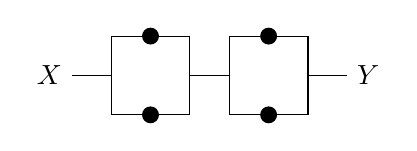
\begin{tikzpicture}
	\draw (0,0) node[anchor=east] {$X$} -- (.5,0) |- (1,.5) -| (1.5,0) -- (2,0) |- (2.5,.5) -| (3,0) -- (3.5,0) node[anchor=west] {$Y$};
\draw (.5,0) |- (1,-.5) -| (1.5,0) -- (2,0) |- (2.5,-.5) -| (3,0);
\filldraw[black] (1,.5) circle (0.1);
\filldraw[black] (1,-.5) circle (0.1);
\filldraw[black] (2.5,.5) circle (0.1);
\filldraw[black] (2.5,-.5) circle (0.1);
\end{tikzpicture}
\begin{enumerate}
\item Przedstaw przestrzeń zdarzeń elementarnych. \ans{$\Omega=\{\omega_{i_1,\ldots,i_4}|i_j\in\{0,1\}\}$}
\item Czy w tej przestrzeni wszystkie zdarzenia elementarne są jednakowo prawdopodobne? \ans{Nie}
\item Jaki jest rozmiar przestrzeni zdarzeń elementarnych? \ans{$\abs{\Omega}=2^4$}
\item Zdefiniuj zdarzenie $A$ jako zbiór zdarzeń elementarnych. \ans{$A=\{
	\omega_{1111},\omega_{1110},\omega_{1101},
		\omega_{1011},\omega_{1010},\omega_{1001},
		\omega_{0111},\omega_{0110},\omega_{0101}
	\}$}
	\item Oblicz prawdpodobieństwo $P(A)$, dbając o to by jasno przedstawić tok rozumowania. \ans{$P(A)=0{,}9^4+4\cdot0{,}9^3\cdot0{,}1+4\cdot0{,}9^2\cdot0{,}1^2=0{,}9801=(0{,}9+0{,}9-0{,}9^2)^2$, np. $P(\omega_{1111})=P(A_1)P(A_2)P(A_3)P(A_4)$}

\end{enumerate}
\end{enumerate}

\clearpage
\section{Zmienne losowe dyskretne jednowymiarowe}
\begin{enumerate}
\item Prawdopodobieństwo trafienia do celu w jednym strzale jest równie $\frac{1}{5}$. Niech $X$ przyjmuje wartość 1 jeżeli udało się trafić i 0 w przeciwnym przypadku.
\begin{enumerate}
\item Podaj rozkład zmiennej losowej $X$. \ans{$P(X=1)=p\quad P(X=0)=1-p$}
\item Oblicz średnią liczbę celnych strzałów. \ans{$EX=p=0{,}2$}
\item Oblicz odchylenie standardowe zmiennej losowej $X$. \ans{$DX=\sqrt{p(1-p)}=0{,}4$}
\item Podaj najbardziej prawdopodobną wartość zmiennej losowej $X$. \ans{$0$}
\end{enumerate}
\item Prawdopodobieństwo trafienia do celu w jednym strzale jest równie $\frac{1}{5}$. Niech $X$ oznacza liczbę strzałów celnych w wykonanej serii 5 niezależnych strzałów. 
\begin{enumerate}
\item Podaj rozkład zmiennej losowej $X$. \ans{$P(X=k)={5 \choose k}\frac{4^{5-k}}{5^5}$}
\item Oblicz prawdopodobieństwo, że liczba strzałów celnych będzie nie mniejsza niż 2. \ans{$P(X\geq 2)=1-P(X=0)-P(X=1)=1-\frac{4^5}{5^5}-5\cdot\frac{4^4}{5^5}=\frac{821}{3125}\approx0{,}263$}
\item Oblicz średnią liczbę celnych strzałów. \ans{$EX=np=1$}
\item Oblicz odchylenie standardowe zmiennej losowej $X$. \ans{$DX=\sqrt{np(1-p)}=\sqrt{\frac{4}{5}}$}
\item Podaj najbardziej prawdopodobną liczbę celnych strzałów. \ans{$\lfloor(n+1)p\rfloor=1$}
\end{enumerate}
\item Linia 64 jeżdżąca na trasie Literacka--Kacza jest obsługiwana przez 7 autobusów, które psują się przypadkowo i niezależnie od siebie. Każdy autobus może w ciągu całego dnia zepsuć się z~prawdopodobieństwem $0{,}25$. Niech $X$ oznacza liczbę autobusów, które w ciągu dnia uległy awarii i musiały zjechać do zajezdni.
\begin{enumerate}
\item Podaj rozkład zmiennej losowej $X$.
\item Oblicz prawdopodobieństwo, że w ciągu całego dnia zepsują się przynajmniej 3 autobusy.
\item Oblicz średnią liczbę zepsutych autobusów.
\item Oblicz odchylenie standardowe zmiennej losowej $X$.
\item Podaj najbardziej prawdopodobną liczbę zepsutych autobusów. \ans{$(n+1)p-1=1, (n+1)p=2$}
\end{enumerate}
\item W Minas Tirith gromadzą zapasy na wypadek oblężenia. Jeżeli mięso,
pakowane w beczki, jest źle wysuszone może się zepsuć. Prawdopodobieństwo, że
tak się stanie wynosi $0{,}0045$ niezależnie dla każdej beczki. W~piwnicach zgromadzono 1000 beczek z mięsem,
niech $X$ oznacza liczbę beczek z zepsutym mięsem.  \begin{enumerate}
\item Podaj rozkład zmiennej losowej $X$. \ans{$P(X=k)={1000\choose k}p^k(1-p)^{1000-k}\approx\frac{\lambda^k}{k!}e^{-\lambda} \quad \lambda=1000\cdot0{,}0045=4{,}5$}
\item Oblicz prawdopodobieństwo, że zepsuje się nie więcej niż 5 beczek. \ans{$P(X\leq 5)=0{,}70290$}
\item Oblicz średnią liczbę zepsutych beczek. \ans{$EX=4{,}5$}
\item Oblicz odchylenie standardowe zmiennej losowej $X$. \ans{$DX=\sqrt{4{,}5}$}
\end{enumerate}
\item Hobbici znani są ze swojej intensywnej i obfitej korespondencji. W Michael
Delving mieszka 500 hobbitów, a~w~ciągu jednego dnia do urzędu pocztowego
przychodzi $X$ hobbitów. Hobbici do urzędu pocztowego przychodzą niezależnie od
siebie i~z~równym prawdopodobieństwem $p$, a~każdego dnia jest ich tam
\emph{średnio} 75. Załóż, że zmienna losowa $X$ ma rozkład dwumianowy.
\begin{enumerate}
\item Oblicz wartość prawdopodobieństwa $p$ przyjścia do urzędu przez pojedynczego hobbita.
\item Podaj  (w formie funkcji prawdopodobieństwa) rozkład prawdopodobieństwa zmiennej losowej $X$.
\item Ile różnych wartości może przyjąć dystrybuanta zmiennej losowej $X$? Odpowiedź uzasadnij.
\item Jaką wartość przyjmie dystrybuanta zmiennej losowej $X$ w punkcie 1000?
\item Oblicz prawdopodobieństwo, że przez cały dzień do urzędu nikt nie przyjdzie.
\item Podaj wartość $EX$.
\item Oblicz odchylenie standardowe zmiennej losowej $X$.
\item Oblicz najbardziej prawdopodobną liczbę hobbitów, którzy przyjdą w ciągu dnia do urzędu.
\end{enumerate}
\clearpage
\item Bilbo bierze udział w grze, w której punkty zdobywa się za trafianie kamykami do celu. Każdemu zawodnikowi przysługuje maksymalnie pięć rzutów, przy czym:
\begin{itemize}
\item na początku każdy zawodnik ma jeden punkt;
\item każdy trafiony rzut powoduje podwojenie liczby posiadanych punktów;
\item rzut nietrafiony oznacza koniec gry dla danego zawodnika.
\end{itemize}
Prawdopodobieństwo, że Bilbo w pojedynczym rzucie trafi do celu wynosi $0{,}7$. Niech $X$ będzie zmienną losową oznaczającą liczbę punktów zdobytych przez
Bilba.
\begin{enumerate}
\item Podaj funkcję prawdopodobieństwa zmiennej losowej $X$.
\item Oblicz dystrybuantę zmiennej losowej $X$.
\item Oblicz $EX$.
\item Oblicz wariancję zmiennej losowej $X$.
\item Oblicz $P(5\leq X\leq 30)$.
\end{enumerate}
\item W piwnicach Brandy Hallu zgromadzono 500 butelek soków na zimę.
Niestety, z poprzednich lat wiadomo, że każda butelka ma $0{,}5\%$ szans nie dotrwać zimy: spleśnieje, skwaśnieje itp.
Niech $X$ będzie zmienną losową oznaczającą liczbę zepsutych butelek soku.
Niech $Y$ będzie zmienną losową oznaczającą liczbę zdatnych do spożycia butelek soku, to znaczy $X+Y=500$.

\begin{enumerate}
\item Podaj funkcję prawdopodobieństwa zmiennej losowej $X$.
\item Podaj wartość średnią i odchylenie standardowe zmiennej losowej $X$.
\item Podaj funkcję prawdopodobieństwa zmiennej losowej $Y$.
\item Podaj wartość średnią i odchylenie standardowe zmiennej losowej $Y$.
\item Podaj najbardziej prawdopodobną liczbę zepsutych butelek.
\item Oblicz prawdopodobieństwo, że liczba przynajmniej 496 butelek soku będzie się nadawało do spożycia.
\item Oblicz prawdopodobieństwo, że liczba zepsutych butelek będzie różniła się od oczekiwanej liczby zepsutych butelek o mniej niż odchylenie standardowe.
\item Oszacuj (z dokładnością do $0{,}1$) prawdopodobieństwo, że liczba butelek nadających się do spożycia przekroczy 300. Odpowiedź uzasadnij.
\end{enumerate}
\item W piwnicy Bamfurlong znajduje się 10 słoików szczególnie cennej konfitury ze świecących gigantycznych pieczarek.
Właściciel przechowuje je na Święto Zimowe, ale nie wie, że ze względu na bliskość rzeki, każdy słoik ma 20\% szans spleśnieć do tego czasu!
Niech $X$ będzie zmienną losową oznaczającą liczbę słoików, które nie zapleśniały do Święta.
Niech $Y$ będzie zmienną losową oznaczającą liczbę słoików, które spleśniały.
Inaczej: $X+Y=10$.

\begin{enumerate}
\item Podaj funkcję prawdopodobieństwa zmiennej losowej $X$.
\item Podaj wartość średnią i odchylenie standardowe zmiennej losowej $X$.
\item Podaj funkcję prawdopodobieństwa zmiennej losowej $Y$.
\item Podaj wartość średnią i odchylenie standardowe zmiennej losowej $Y$.
\item Podaj najbardziej prawdopodobną liczbę zepsutych słoików.
\item Oblicz prawdopodobieństwo, że przynajmniej 8 słoików będzie się nadawało do spożycia.
\item Oblicz prawdopodobieństwo, że liczba zepsutych słoików będzie różniła się od oczekiwanej liczby zepsutych słoików o mniej niż odchylenie standardowe.
\end{enumerate}

\end{enumerate}


\end{document}
